\chapter{Notions mathématiques}

Nous allons traiter dans cette section de notions mathématiques qui seront abordées dans la suite de ce mémoire. Ce sont des notions importantes pour notre bonne compréhension du sujet et de ses enjeux.

\section{Métriques et Espaces métriques}

\subsection*{Métriques}
Une métrique est une mesure de distance, c'est une fonction qui retourne la distance entre deux points. Dans le plan cartésien, on sait que la distance entre deux points $(x_1, y_1)$ et $(x_2, y_2)$ est donnée par la formule de distance : \\
$$ \sqrt{(x_2 - x_1)^2 - (y_2 -y_1)^2} $$

%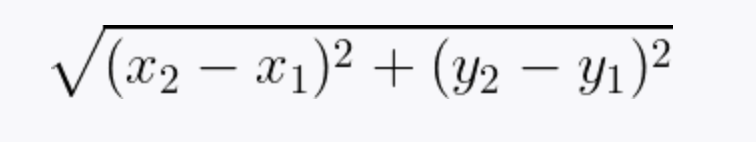
\includegraphics[width=100pt]{./img/notions_math/metric/eq_cartesienne}


C'est généralement la façon dont nous pensons à la distance. Mais dans de nombreuses situations réelles, nous ne pouvons pas penser à nos points de données d'une manière qui aurait le sens géométrique.
\\
Par exemple, imaginons que nous avons une courbes de prix des actions de deux sociétés différentes. Disons que $f(t)$ est une fonction représentant le prix d'une action au temps $t$ et $g(t)$ représente le prix d'une autre action au temps $t$. Quelle est la distance entre les fonctions $f$ et $g$ ? 
\\
Pour répondre à cette question, nous ne pouvons pas utiliser la formule de distance vu précedemment. Nous avons besoin d'une définition plus générale. 
\\
\\
Supposons que $X$ soit un ensemble quelconque. Nous définissons une métrique sur $X$ comme une fonction de distance $d$ qui satisfait les axiomes suivants :
\begin{enumerate}
        \item $d(x, x)=0$ pour tout $x \in X$
        \item $d(x, y)=d(y, x)$ pour tout $x,y \in X$
        \item $d(x, y) \geqslant 0$ pour tout $x, y, z \in X$
        \item $d(x, y) \leqslant d(x, z) + d(z, y)$ pour tout $x, y, z \in X$
\end{enumerate}

Le premier axiome signifie que chaque élément de x est à une distance 0 de lui-même. Le deuxième axiome signifie que la distance de x à y est la même que la distance de y à x. Puisque la distance négative n'a pas de sens, le troisième axiome garantit que deux points n'ont pas de distance négative l'un par rapport à l'autre. Le dernier axiome, et le plus important, est connu sous le nom d'inégalité triangulaire. La règle du triangle est l'une des inégalités les plus importantes des mathématiques, malgré sa simplicité. Elle stipule essentiellement que la somme des deux côtés d'un triangle est supérieure à l'un de ses côtés.
\\
\\
Nous allons examiner quelques métriques intéressantes pour mieux comprendre l'intérêt d'utiliser des métriques différentes. Elles vérifient évidement toutes les précedents axiomes.


\textbf{Métrique discrète}
\\
Pour tout ensemble $X$, la métrique discrète est définie comme suit :

%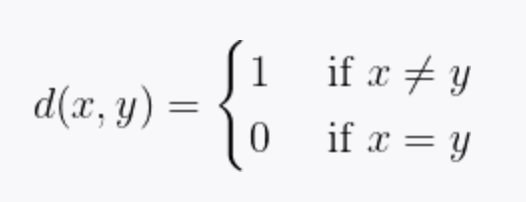
\includegraphics[width=100pt]{./img/notions_math/metric/metric_discret}
\[ d(x,y) =
  \begin{cases}
    1       & \quad \text{si } x \ne y \\
    0       & \quad \text{si } x = y 
  \end{cases}
\]



\textbf{Valeur absolue}
\\
Dans $\mathbb{R}$, l'ensemble de tous les nombres réels, la fonction : 

%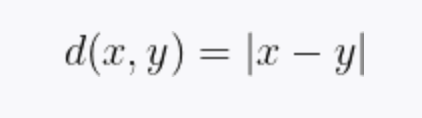
\includegraphics[width=100pt]{./img/notions_math/metric/val_abs}
$$ d(x,y) = \lvert x - y \rvert$$

\textbf{Fonction continue}
\\
Soit $C[0, 1]$ l'espace des fonctions continues avec le domaine [$0, 1]$. Il existe plusieurs métriques que l'on peut placer sur cet espace :

%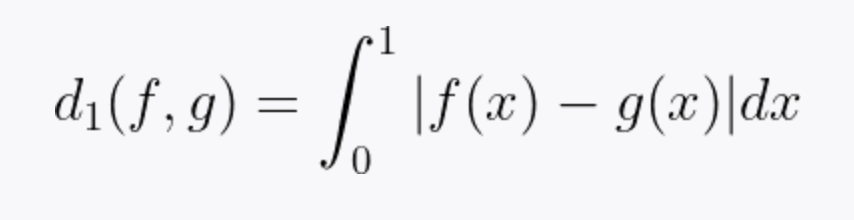
\includegraphics[width=100pt]{./img/notions_math/metric/eq_fcn_con_1_1}
$$ d_1(f,g) = \int_0^1  \lvert f(x) - g(x) \rvert dx$$


Cela définit l'aire totale entre deux fonctions $f$ et $g$ : 


\begin{figure}[h!]
  \caption{Titre de la figure (source : \cite{arrow48})}
  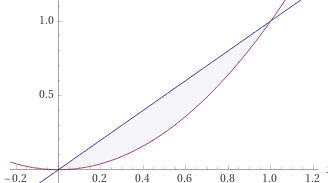
\includegraphics[width=200pt]{./img/notions_math/metric/courbe_metric_fcn}
\end{figure}

En général, si f et g sont deux fonctions dans C[a, b], alors on définit pour tout p >= 1 :

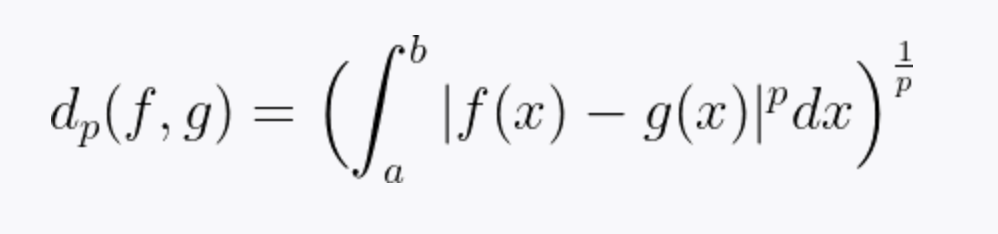
\includegraphics[width=100pt]{./img/notions_math/metric/eq_fcn_con_1_2}
\\
\\
\textit{Une autre métrique continue}
\\
Soit C[a, b] l'espace des fonctions continues avec le domaine [a, b]. Nous pouvons définir la métrique suivante comme êtant la distance maximale entre f et g dans l'intervalle [a, b] : 
\\
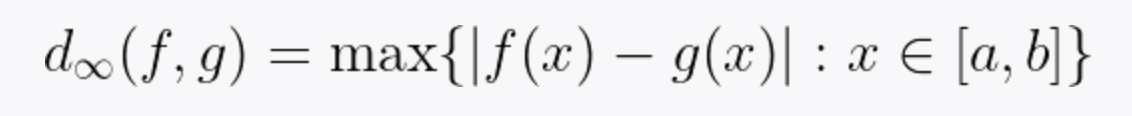
\includegraphics[width=100pt]{./img/notions_math/metric/eq_fcn_con_2}


    
\section*{Espaces Métrique}
Maintenant que nous avons une idée de ce qu'est une métrique, nous pouvons définir les espaces métriques. Un espace métrique est une paire (X, d) où X est un ensemble, et d est une métrique définie sur des points de l'ensemble X. Nous venons de voir plusieurs exemples d'espaces métriques ci-dessus. Nous allons maintenant examiner certaines propriétés importantes des espaces métriques.
\\
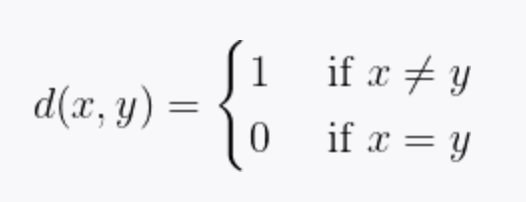
\includegraphics[width=100pt]{./img/notions_math/metric/metric_discret.png}
\\
Soit (X, d) un espace métrique, et soit $x_0$ un élément quelconque de X. Pour un certain $r > 0$ fixé, définissez la boule ouverte de rayon r centrée sur $x_0$ par l'ensemble ci-dessous (aussi écrit $B(x_0 ; r)$): 
\\
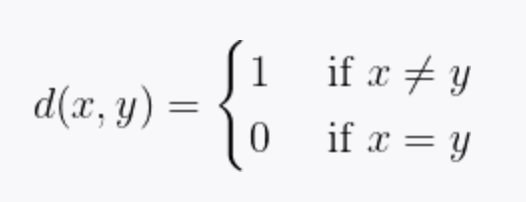
\includegraphics[width=100pt]{./img/notions_math/metric/metric_discret.png}



\section*{Cosine Distance}
Nous allons nous intésser à la distance cosinus (ainsi  qu'à la similarité cosinus). En effet, comme nous allons le  voir plus tard, cette mesure peut être intéressantes dans notre utilisation de UMAP. En effet, nous verrons que le choix de la métrique peut avoir une influence intéressante sur l'algorithme et nous allons essayer de comprendre pourquoi cette métrique peut être particulièrement adapté à notre problème (ou pas).
\\
\\
Pour commencer nous allons définir la similarité en cosinus. Il s'agit d'une métrique qui mesure le cosinus de l'angle entre deux vecteurs projetés dans un espace multidimensionnel.


Plus l'angle entre les deux vecteurs est petit, plus ils sont similaires l'un à l'autre; Donc plus la similarité cosinus se rapproche de 1, plus l'angle entre les deux vecteurs A et B est faible. Dans ce cas, A et B sont plus similaires l'un à l'autre.
\\
Supposons maintenant que l'angle entre les deux vecteurs soit de 90 degrés, la similitude en cosinus aura une valeur de 0. Cela signifie que les deux vecteurs sont perpendiculaires l'un à l'autre, ce qui signifie qu'il n'y a aucune corrélation entre eux.
\\
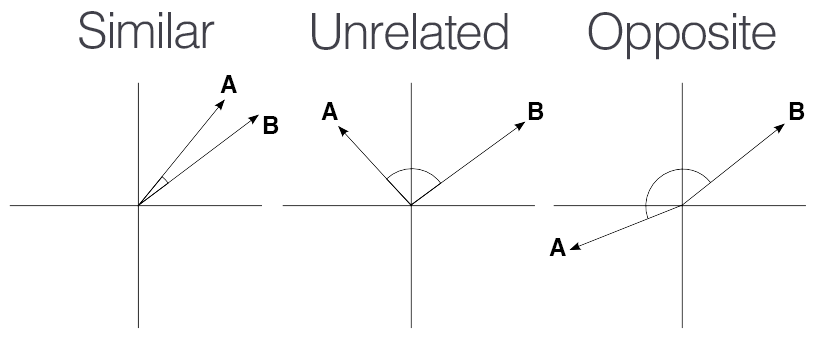
\includegraphics[width=200pt]{./img/notions_math/metric/img_metric_cos.png}


La similarité en cosinus est décrite mathématiquement comme la division entre le produit scalaire des vecteurs et le produit des normes euclidiennes ou de la magnitude de chaque vecteur :


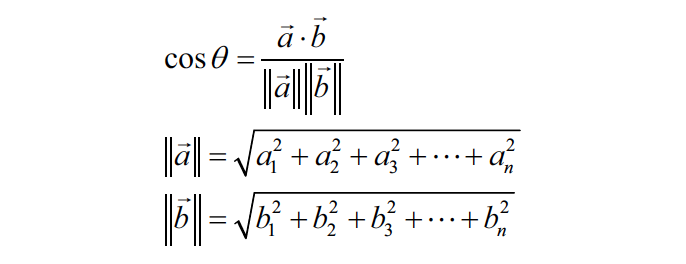
\includegraphics[width=200pt]{./img/notions_math/metric/eq_metric_cos.png}
\\
Où, a et b sont des vecteurs dans un espace multidimensionnel.


Puisque la valeur $\cos(\theta)$ est comprise dans l'intervalle [-1,1] :
\begin{itemize}
    \item La valeur -1 indiquera des vecteurs fortement opposés, c'est-à-dire aucune similarité.
    \item 0 indique des vecteurs indépendants (ou orthogonaux).
    \item 1 indique une forte similarité entre les vecteurs.
\end{itemize}
La distance cosinus est définit comme :
\begin{eqnarray}
    Cosine Distance = 1 — Cosine Similarity
\end{eqnarray}
L'intuition derrière cela est que si 2 vecteurs sont parfaitement identiques alors la similarité est de 1 (angle=0 donc $\cos(\theta)$=1) et donc, la distance est de 0 (1-1=0).
\\
\\
La distance du cosinus est utilisée dans de nombreux domaines, par exemple :
\begin{enumerate}
    \item Cette métrique est utilisée dans les processus d'exploration de données, de recherche d'informations et de mise en correspondance de textes.
    \item Elle est aussi utilisé dans les moteurs de recommandation pour recommander des produits/films/spectacles/livres similaires.
    \item Dans le domaine de la recherche d'informations, l'utilisation de TF-IDF pondéré et de la similarité en cosinus est une technique très courante pour retrouver rapidement les documents similaires à une requête de recherche.
\end{enumerate}



\newpage







\section{Fléau de la dimension}
De nombreux jeux de données impliquent des milliers, voire des millions de caractéristiques pour chaque observation. Toutes ces caractéristiques peuvent rendre l'apprentissage extrêmement lent, mais elles peuvent aussi rendre beaucoup plus difficile la recherche d'une bonne solution. Ce problème est souvent appelé fléau de la dimension.
\\
Si nous avons plus de caractéristiques que d'observations, nous courons le risque de surajuster massivement (overfitting) notre modèle. Cela ce traduit généralement par des performances hors échantillon épouvantables.
\\
Lorsque nous avons trop de caractéristiques, les observations deviennent plus difficiles à regrouper. Trop de dimensions font que chaque observation du jeu de données semble équidistante de toutes les autres. Et comme le clustering utilise une mesure de distance telle que la distance euclidienne pour quantifier la similarité entre les observations, c'est un gros problème. Si les distances sont toutes approximativement égales, alors toutes les observations semblent également similaires (ainsi qu'également différentes), et aucun cluster significatif ne peut être formé.
\\
\\
Le fait d'avoir trop de caractéristiques peut perturber certains algorithmes de machine learning tels que les algorithmes de clustering. La réduction de la dimensionnalité peut aider à améliorer les performances de ceux-ci.
\\
Dans le monde réel les données souvent désordonnées avec du bruit et des relations compliquées. La réduction de la dimensionnalité représente un compromis entre un modèle potentiellement plus robuste et une interprétabilité moindre.
\\
\\
\\
\\
Georg Cantor est un mathématicien allemand du 19e siècle qui est particulièrement connu pour son travail sur la théorie des ensembles et plus spécifiquement sur ses résultats concernant l’infini. L’ensemble des nombres entier est infini par construction, mais l’ensemble des nombres entier relatif également. Et intuitivement, nous nous disons que ces infini ne sont pas vraiment les mêmes, puisqu’il semblerait que Z soit plus grand que N ! Georg Cantor montre que ces deux infini sont en fait les mêmes : il y a autant de nombres dans Z que dans N. Plus fort encore, il démontre la puissance de l’infini qui nous donne un résultat encore plus contre intuitif : il y a autant de nombre dans l’interval $[0, 1]$ que dans R tout entier ! Alors qu’il venait de le démontrer, il a envoyé une lettre à son ami mathématicien Dedekind :
\begin{quotation}
    Tant que vous ne m’aurez pas approuvé, je ne puis que dire : je le vois mais je ne le crois pas.
    \\
    Georg Cantor (1877)
\end{quotation}
Il a prouvé quelque chose que l’ensemble de la communauté pensait intuitivement fausse, et lui-même n’y croyait pas. Nous sommes toujours mis en difficulté quand il s’agit de traiter avec l’infini, ou des grandes quantités. Cette remarque nous amène donc à nous questionner sur l’impact d’un grand nombre d’informations quand nous entraînons un modèle de Machine Learning.
\\
\\
Le fléau de la dimension est un phénomène connu en statistique et en Machine Learning. Ce terme rassemble tout un ensemble de phénomène qui se produisent en très grande dimension, mais pas dans une dimension plus petite. Nous proposons dans cette annexe d’illustrer quelque-uns des phénomènes étranges de la grande dimension et ses impacts en Machine Learning.
\begin{quotation}
    The curse of dimensionality is taught in every Machine Learning programs, and refers to \textit{various phenomea that arise when analyzing and organizing data in high-dimensional spaces that do not occur in low-dimensional settings}\footnote{Definition from Wikipedia}. Living in a three dimensional world, it is known to be hard for human to apprehend infinity\footnote{e.g. the Cantor's work in mathematics with infinite set in set theory.}. Not fully understanding what the curse of dimensionality was as a student, I decided to look for strange behavior in high-dimension, hoping that it would shed light on the dimension curse.
\end{quotation}
\textbf{Volume d’une hypersphère}
Pour essayer de sentir les problèmes de la très grande dimension, on s’intéresse au volume d’une hypersphère.
\\
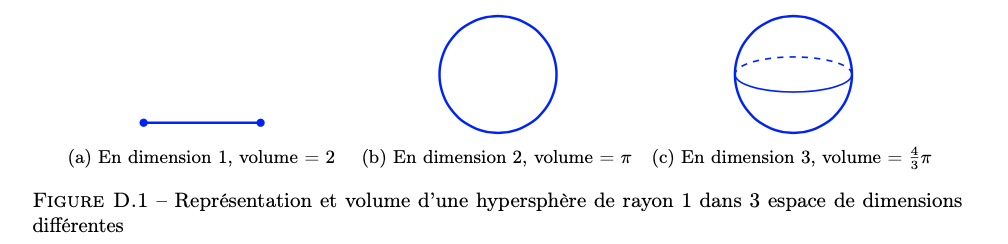
\includegraphics[width=\linewidth]{./img/notions_math/hypersphere_1}
\\
Avec la figure ci-dessus nous avons l’intuition que le volume augmente avec la dimension. Donc pour une hypersphère de très grande dimension, on devrait avoir un très grand volume.
\\
Nous avons tracé et mesuré le volume pour la distance euclidienne classique, mais nous pouvons aussi utiliser d’autre distance (autre norme) comme montré dans la figure ci-dessous.
\\
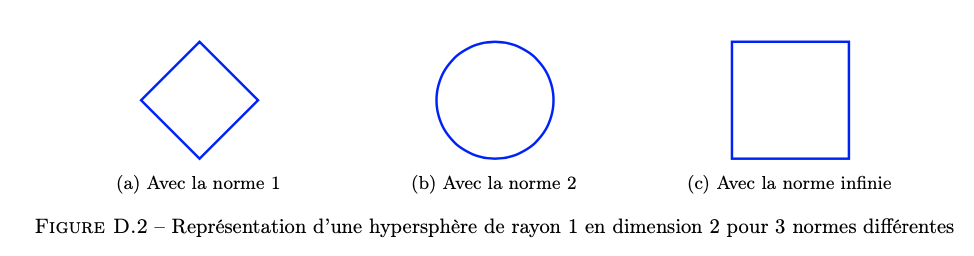
\includegraphics[width=\linewidth]{./img/notions_math/hypersphere_2}
\\
Formalisons le problème et généralisons-le pour calculer le volume d’une hypersphère en n’importe quelle dimension et pour n’importe quelle norme. Soit $n \in \mathbb{N}^*$ la dimension de l’espace, on appelle boule ou hypersphère l’objet défini par :

\begin{eqnarray*} 
    B_n^p(R) &=& \{ (x_1, \ldots, x_n) \in \mathbb{R}^n, \sum_{i=1}^n x_i^p \leqslant R^p\} \\
    &=& \{ u \in \mathbb{R}^n, \|u\|_p^p \leqslant R^p\}
\end{eqnarray*}

Nous savons que $\|u\|_p$ est la norme $p$ définit comme $\|u\|_p^p=\sum_{i=1}^n x_i^p$. $B_n^p(R)$ est la boule de dimension $n$ avec une norme $p$ de rayon $R$. On définit $V_n^p(R)$ le volume de la boule $B_n^p(R)$ \textit{i.e.} la measure de $B_n^p(R)$ pour la mesure de Lesbegue dans $\mathbb{R}^n$. Formellement :
\\
\begin{equation*} V_n^p(R) = \int_{B_n^p(R)} \bigotimes_{i=1}^n\mathrm{d}x_i \end{equation*}
\\
On définit la focntion:
\\
\begin{equation*}
\begin{array}{ccccc}
\phi & : & B_n^p(1) & \to & B_n^p(R) \\
& & (x_1, \ldots, x_n) & \mapsto & (Rx_1, \ldots, Rx_n) \\
\end{array}
\end{equation*}
Nous avons cela pour $u\in B_n^p(1)$, ensuite $\|u\|_p^p \leqslant 1 \Longleftrightarrow \|Ru\|_p^p \leqslant R^p$ donc $\phi(u) \in B_n^p(R)$, sous l'hypothèse $R>0$. 
Par équivalence, nous avons $\phi(B_n^p(1)) = \phi(B_n^p(R)$. $\phi$ est alors une correspondance biunivoque, alors par changement de variable on a : $V_n^p(R) = R^nV_n^p(1)$.
\\
Donc par Fubini :
\begin{eqnarray*}
V_n^p(1) &=& \int_{-1}^1 V_{n-1}^p\left(\sqrt[p]{1 - |x|^p}\right)\mathrm{d}x\\
&=& V_{n-1}^p(1) \int_{-1}^1 \left(1-|x|^p\right)^{\frac{n-1}{p}} \mathrm{d}x\\
&=& 2V_{n-1}^p(1) \int_0^1 \left(1-|x|^p\right)^{\frac{n-1}{p}} \mathrm{d}x\\
&=& \frac{2}{p} V_{n-1}^p(1) \int_0^1 y^{\frac{1}{p}-1}(1-y)^{\frac{n-1}{p}}\mathrm{d}y\\
\end{eqnarray*}
On rappelle la définition de la fonction Bêta définie pour $x, y \in \mathbb{R}_+^*$ :
\begin{equation*} B(x, y) = \int_0^1 t^{x-1}(1-t)^{y-1}\mathrm{d}t \end{equation*}
Nous connaissons aussi l'identité :
\begin{equation*} B(x, y) = \frac{\Gamma(x) \Gamma(y)}{\Gamma(x+y)} \end{equation*}

\textbf{La fonction Bêta}
\\
\\
Nous prouvons ici l'identité que nous avons utilisée pour trouver l'expression exacte du volume d'une boule en dimension $n$ en utilisant la distance $p$-normale. La fonction bêta est définie comme dit précédemment :
\\
\begin{equation*} B(x, y) = \int_0^1 t^{x-1}(1-t)^{y-1}\mathrm{d}t \end{equation*}
Pour $x,y > 0$. Et nous utilisons l'identité suivante :

%\lemme{Let $x, y \in \mathbb{R}_+^*$, we have :

%\begin{equation*} B(x, y) = \frac{\Gamma(x) \Gamma(y)}{\Gamma(x+y)} \end{equation*}
%}
\begin{proof}
Nous avons :

\begin{eqnarray*}
\Gamma(x)\Gamma(y) &=& \int_0^{+\infty} e^{-a}a^{x-1}\mathrm{d}a \times  \int_0^{+\infty} e^{-b}b^{x-1}\mathrm{d}b\\
&=& \int_{a=0}^{+\infty} \int_{b=0}^{+\infty} e^{-(a+b)}a^{x-1}b^{y-1}\mathrm{d}b\mathrm{d}a
\end{eqnarray*}

Nous effectuons le changement de variables : $u=a+b$ et $\displaystyle v=\frac{a}{a+b}$, qui est équivalent à $a=uv$ et $b=u(1-v)$. Nous avons maintenant :
\\
\begin{eqnarray*}
\Gamma(x)\Gamma(y) &=& \int_0^1\int_0^{+\infty} (uv)^{x-1}\left[u(1-v)\right]^{y-1}e^{-[uv+u(1-v)]}|-u|\mathrm{d}u\mathrm{d}v\\
&=& \int_0^1\int_0^{+\infty}u^{x+y-1}v^{x-1}(1-v)^{y-1}e^{-u}\mathrm{d}u\mathrm{d}v\\
&=& \int_0^1 v^{x-1}(1-v)^{y-1}\mathrm{d}v \times \int_0^{+\infty}u^{x+y-1}e^{-u}\mathrm{d}u\\
&=& B(x, y)\Gamma(x+y)
\end{eqnarray*}
\end{proof}



Nous pouvons alors écrire :
\begin{eqnarray*}
V_n^p(1) &=& \frac{2}{p} V_{n-1}^p(1) \frac{\Gamma\left(\frac{1}{p}\right)\Gamma\left(\frac{n-1}{p}+1\right)}{\Gamma\left(\frac{n}{p} + 1\right)}
\\
&=& V_{n-1}^p(1) \left[\frac{2}{p} \frac{\Gamma\left(\frac{1}{p}\right)\Gamma\left(\frac{n-1}{p}+1\right)}{\Gamma\left(\frac{n}{p} + 1\right)} \right]
\\
&=& V_1^p(1)2^{n-1}\Gamma\left(\frac{1}{p}+1\right)^{n-1} \frac{\Gamma\left(\frac{1}{p}+1\right)}{\Gamma\left(\frac{n}{p}+1\right)}
\\
&=& V_1^p(1)2^{n-1}\frac{\Gamma\left(\frac{1}{p}+1\right)^n}{\Gamma\left(\frac{n}{p}+1\right)}
\\
\end{eqnarray*}
Depuis $V_1^p(1) = 2$, nous obtenons la formule finale : 
\begin{equation*} \forall n\geqslant 2, \forall p\geqslant 1,  \; \; \;  V_n^p(1) = \frac{\left(2\Gamma\left(\frac{1}{p}+1\right)\right)^n}{\Gamma\left(\frac{n}{p}+1\right)} \end{equation*}
Donc avec un rayon, nous avons :
\\
\begin{equation} \forall R>0, \forall n\geqslant 2, \forall p\geqslant 1, \; \; \; V_n^p(R) = \frac{\left(2R\Gamma\left(\frac{1}{p}+1\right)\right)^n}{\Gamma\left(\frac{n}{p}+1\right)} \end{equation}
Nous aimerions savoir comment il se comporte en haute dimension, \textit{i.e.} pour $n$ assez grand. Nous savons que $\Gamma(n+1) = n!$ pour tout $n\in\mathbb{N}$. Donc nous utilisons cela pour l'équivalence :
\\
\begin{equation} 
V_n^p(R) \sim \sqrt{\frac{p}{2\pi n}} \left[2R\Gamma\left(\frac{1}{p}+1\right) \left(\frac{pe}{n}\right)^{\frac{1}{p}}\right]^n 
\end{equation}




Ce que ce résultat exhibe, c’est que le volume d’une hypersphère en grande dimension tend exponentiellement vite vers 0, c’est complètement contre intuitif ! Traçons des courbes de cette fonction :
\\
\\
Tout d'abord, nous voyons le premier fait surprenant : le volume qui augmente avec n converge vers 0 pour toute dimension métrique p ou tout rayon R. Avec notre intuition dans un monde tridimensionnel, nous nous attendions à ce que le volume augmente à l'infini. On peut regarder différentes courbes :
\\
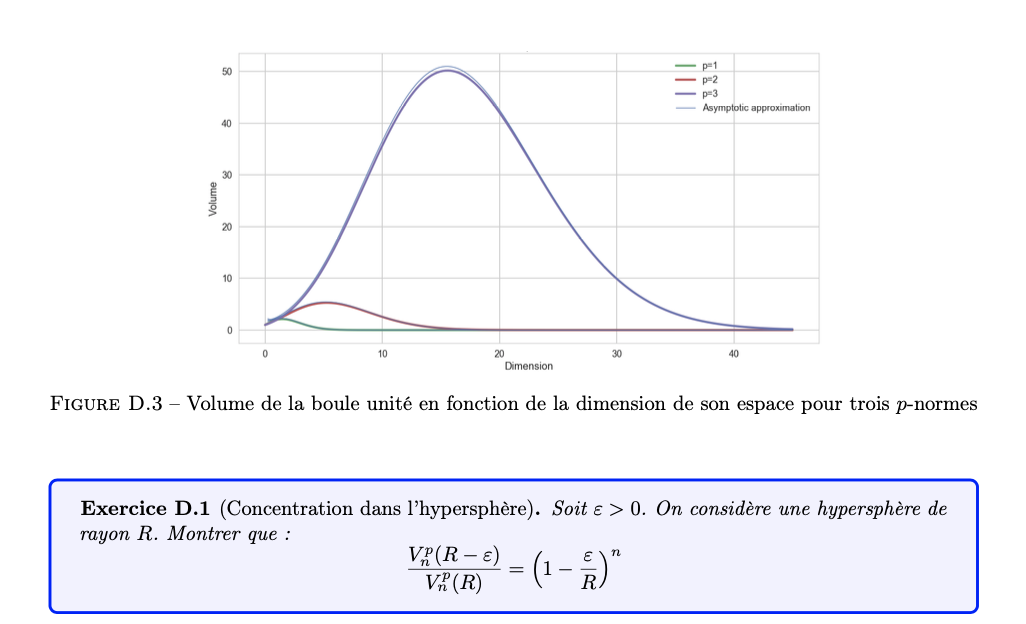
\includegraphics[width=\linewidth]{./img/notions_math/courbe}
\\
On retrouve bien le comportement en hausse que nous avions observé, mais on comprend que le comportement ultime est que le volume tende vers 0 très rapidement. Avant de discuter de ce que ce résultat implique, regardons un autre résultat contre intuitif.
\\
\\
Nous obtenons ici la vérification graphique que nos calculs pour l'approximation semblent corrects. Nous voyons également qu'ils ont la même forme, mais à une échelle très différente. Nous voyons notre premier fait contre intuitif sur la haute dimension : le volume d'une boule de rayon R tendra toujours vers zéro quand la dimension augmentera. La vitesse de convergence dépend à la fois de R et de l'ordre de la norme que nous prenons.
\\
\\
\textbf{Concentration dans l’hypersphère}
\\
Soit $\epsilon$ > 0. On considère une hypersphère de rayon R. Montrer que :
\\
\\
Un autre fait contre intuitif que l'on peut facilement regarder, est que l'essentiel du volume d'une boule est situé dans un minuscule anneau proche de la frontière. En effet, on peut voir que le rapport entre le volume d'une boule de rayon$R-\varepsilon$ et le volume d'une boule de rayon $R$ en dimension $n$ est :
\begin{equation*} \frac{V_n^p(R - \varepsilon)}{V_n^p(R)} = \left(1- \frac{\varepsilon}{R}\right)^n \end{equation*}
C’est encore plus étrange : les points semblent se concentrer proche des frontières de l’hypersphère, donc en ayant un centre vide. Cela veut dire que plus la dimension augmente, plus le volume tend vers 0 et que dans le même temps les données se rapproche des frontières.
\\
Donc si l’on distribue des points uniformément dans une sphère, la distribution des distances entre les points ne sera pas informative du tout. Ces intuitions sont confirmés par la figure ci-dessous.
\\
\\
Toutefois, lorsque $n$ augmente, le ratio converge rapidement vers 0 avec $\varepsilon$ petit. Pour la boule unitaire de dimension $n=100$, 63\% du volume est dans l'anneau de largeur $\varepsilon = 0.01$.
\\
Ensuite, pour la norme euclidienne, si le volume converge vers zéro, mais que la distance maximale entre deux points reste à $2R$ et que la majeure partie du volume est dans un minuscule anneau, la distribution entre les distances par paire ne devrait pas être uniforme même si les points sont tirés au hasard à l'intérieur d'une boule. Nous avons effectué plusieurs tests sur Python :
\\
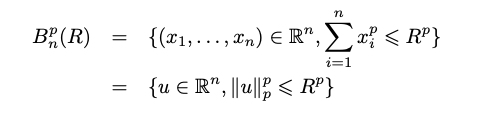
\includegraphics[width=\linewidth]{./img/notions_math/courbe_2}
\\
Ainsi, plus la dimension est grande, moins la notion de distance a du sens. Au delà de l’aspect combinatoire et de stockage des données, avoir un modèle qui a moins d’indicateurs pour s’entraîner aura plus de chance d’être performant et utile. Par exemple, l’ensemble des méthodes de clustering par exemple seront largement impacté par une très grande dimension. Finalement, on peut remettre en cause l’exactitude d’une idée répandue : "Avec plus d’informations les modèles sont meilleurs". Ce qui est plus exact est qu’avec les informations utiles, les modèles sont meilleurs. C’est tout l’enjeux de la phase exploratoire et d’augmentation des données pour répondre à un problème de Machine Learning.
\\
\\
Un deuxième problème majeur en grande dimension est que le nombre de donnée à obtenir pour être capable d’avoir des garanties statistiques sur la qualités de l’apprentissage est colossal, c’est exponentiel. Ainsi, on peut se poser la question de la capacité des algorithmes à apprendre en grande dimension.
\\
\\
Avec cette dernière information, nous comprenons que plus la dimension est élevée, plus les distances sont insignifiantes. Par conséquent, lorsque l'on tente de construire un modèle, il faut toujours rechercher un nombre réduit de variables explicatives et mettre l'accent sur l'utilité des variables. Ce dernier conseil est encore plus important lorsque l'apprentissage automatique est utilisé pour aider d'autres personnes qui ne savent pas ce qu'est l'apprentissage automatique, cela simplifiera grandement l'échange et la collaboration.
\\
\\





\textbf{Interpolation et extrapolation}
\\
\\
L’ensemble du Machine Learning tel qu’on l’a présenté correspond à de l’interpolation et à essayer de faire en sorte que cette interpolation puisse être capable d’extrapoler correctement. Randall Balestriero, Jerome Pesenti et Yann Le Cun on publié en 2021 l’article Learning in High Dimension always amount to extrapolation dont voici le résumé :
\begin{quotation}
    The notion of interpolation and extrapolation is fundamental in various fields from deep learning to function approximation. Interpolation occurs for a sample x whenever this sample falls inside or on the boundary of the given dataset ?s convex hull. Extrapolation occurs when x falls outside of that convex hull. One fundamental (mis)conception is that state-of-the-art algorithms work so well because of their ability to correctly interpolate training data. A second (mis)conception is that interpolation happens throughout tasks and datasets, in fact, many intuitions and theories rely on that assumption. We empirically and theoretically argue against those two points and demonstrate that on any high-dimensional (>100) dataset, interpolation almost surely never happens. Those results challenge the validity of our current interpolation/extrapolation definition as an indicator of generaliza- tion performances.
    \\  
    Randall Balestriero, Jerome Pesenti et Yann Le Cun (2021)
\end{quotation}
L’objet de l’article est de montrer que l’on comprend et défini mal les notions d’interpolation et d’extrapolation en Machine Learning. Cela a des impacts théorique et donc pratique sur notre conception et les garanties mathématiques que l’on peut avoir sur les comportements des algorithmes présenté en très grande dimension. Nous invitons à lire en détail cet article pour en apprendre plus sur le sujet en lui-même, mais également pour voir qu’un domaine qui semble plutôt bien établi et en constante expansion se pose encore des questions sur ses fondements.
\\
\\
En résumé, le fléau de la dimension met en lumière les limites de notre intuition humaine et nous amène à nous questionner encore aujourd’hui sur les fondements communément accepté. Être capable de répondre à ces questions nous permettrait d’être plus précis et plus complet sur notre approche de l’apprentissage en grande dimension.
\\
De manière plus pragmatique, un data scientist doit être au courant que ces questions existent et que le fléau de la dimension va impacter son travail. D’où les techniques de réduction de dimension qui aide à résoudre le problème, mais ne le résolve clairement pas par construction.


    
\newpage






\section{Descente de gradient}
La descente de gradient est une méthode d’optimisation numérique qui s’applique dans de très nombreux domaine. Pour appliquer cette méthode, il faut que nous ayons un problème qui puisse s’écrire sous la forme suivante, avec une fonction $f$ différentiable :
\begin{eqnarray*}
    x^* = \underset{x \in \mathbb{R}^d}{\mathrm{argmin}}\, f(x)
\end{eqnarray*}
Cela ressemble complètement aux différents problèmes que nous avons rencontré jusqu’ici ! La méthode de descente de gradient est une méthode itérative qui va approcher la solution en appliquant la suite :
\begin{eqnarray*}
    x_{t+1} = x_t - \eta \nabla f(x_t)
\end{eqnarray*}
A chaque itération, nous allons nous déplacer dans la direction opposée à la valeur du gradient. Visuellement :
\\
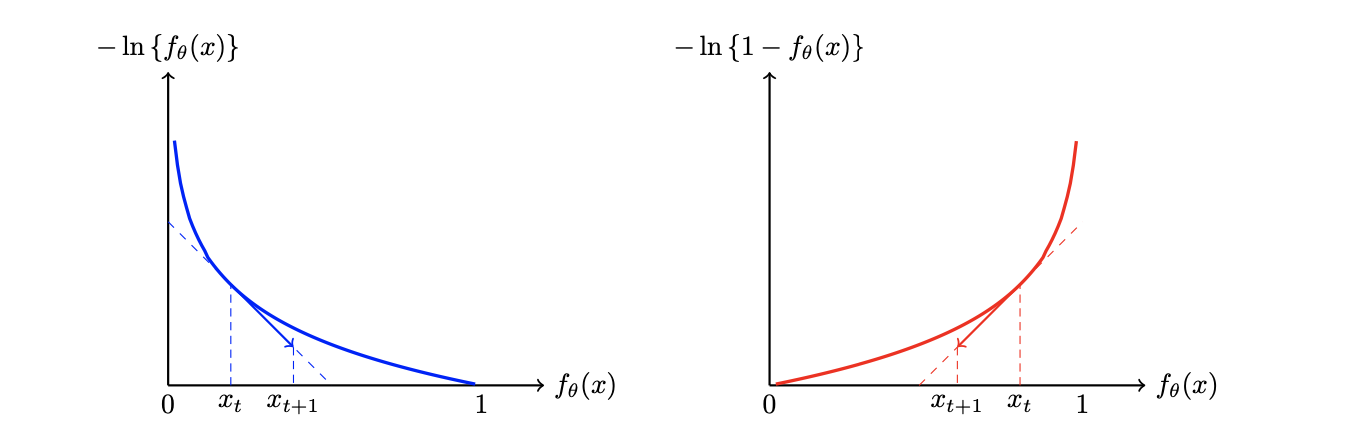
\includegraphics[width=\linewidth]{./img/notions_math/gradiant_descent/courbe_1}
\\
Chaque itération on descend le gradient et l’on s’approche ainsi du minimum de la fonction. Si l’on choisi $x_{t+1}$ comme le point où la tangente croise $y = 0$, alors on obtient l’algorithme de Newton-Raphson qui est également un algorithme d’optimisation. Il est différent de la descente de gradient, car la descente de gradient ne cherche pas à aller jusqu’à $y = 0$ : il va dans cette direction mais parcours $\eta \nabla f(x_t)$ dans cette direction.
\\
\\
En deux dimension, on ne traite plus d’une courbe dont on cherche le minimum comme nous le voyions dans les premiers exemples. On traite ici d’une surface en deux dimensions où l’on cherche les coordonnées du point minimal. Dans la figure (3.2) on voit comment la descente se comporte en plaçant un point à chaque itération.
\\
Le paramètre $\eta$ est crucial dans la descente de gradient, c’est le learning rate. Son rôle est de contrôler l’amplitude des pas de descente. Toujours dans la figure en deux dimensions, on remarque que les points sont de plus en plus rapprochés. La descente de gradient est de moins en moins brusque, et on modifie que très peu le paramètre dans les dernières itérations. Voyons sur l’exemple (3.3) en une seule dimension comment se comporte la descente de gradient en fonction de la valeur de $\eta$.
\\
Le learning rate contrôle la vitesse de convergence vers le minimum (s'il existe), il doit être bien choisit sinon on s’expose à deux problèmes :
\\
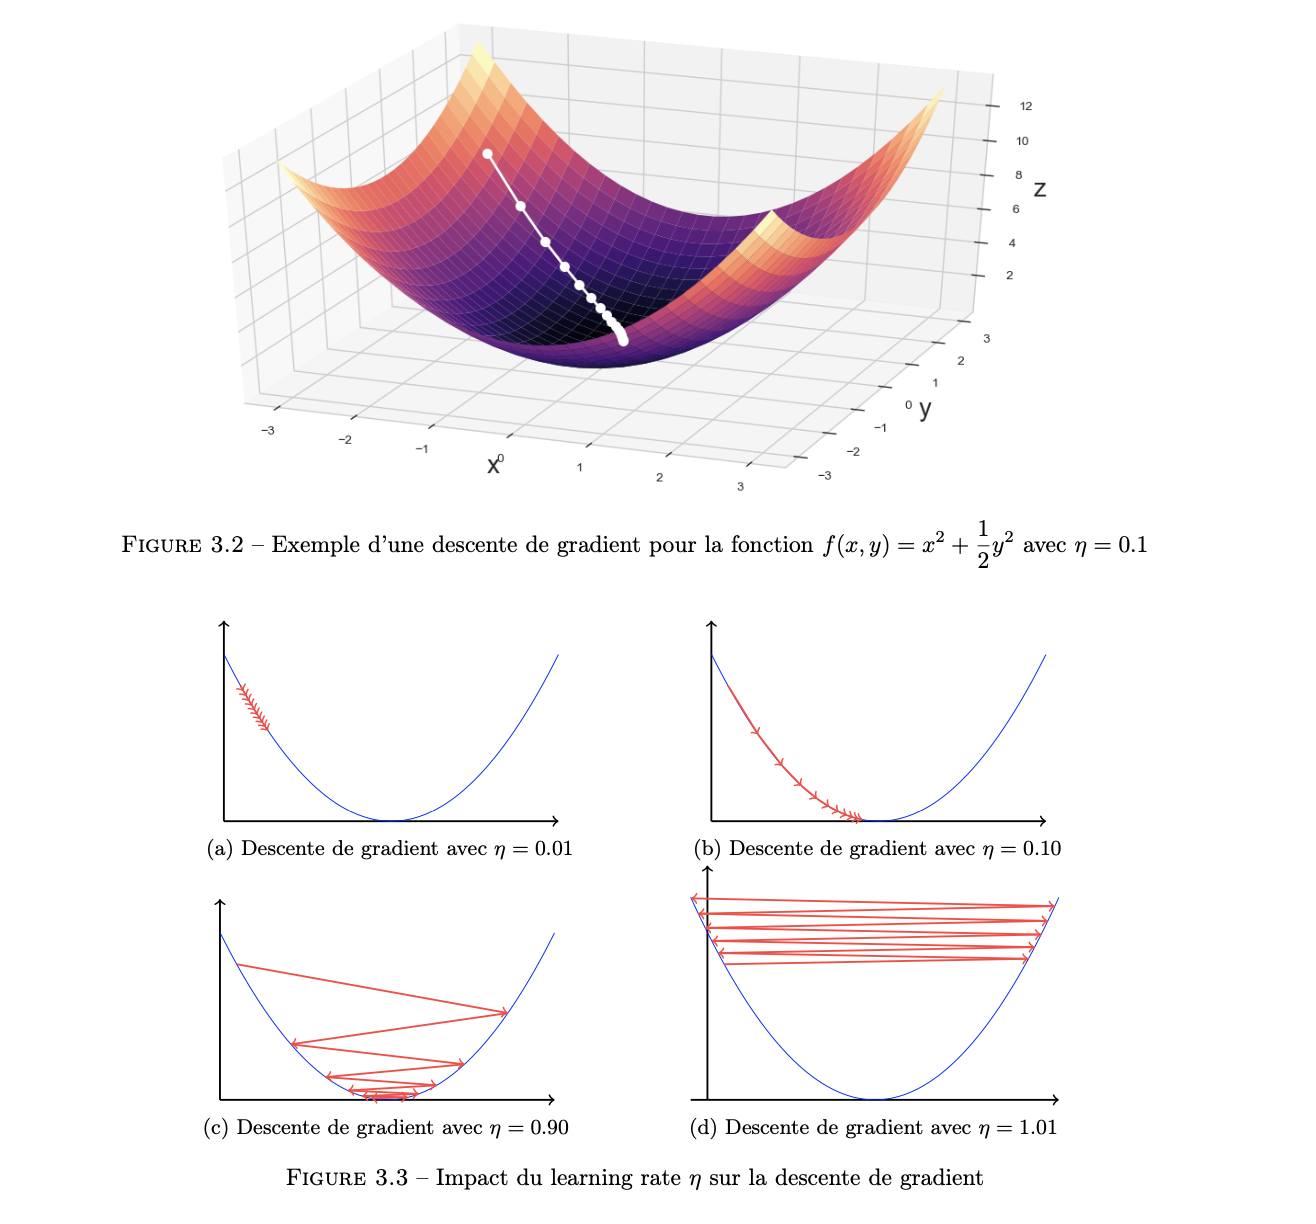
\includegraphics[width=\linewidth]{./img/notions_math/gradiant_descent/courbe_2}
\begin{itemize}
    \item On descend trop doucement : le learning rate est trop faible. C’est le cas de la première descente de gradient (3.3a).
    \item On ne descend pas et on diverge : le learning rate est trop fort. C’est le cas de la dernière descente de gradient (3.3d).
\end{itemize}
La deuxième descente de gradient (3.3b) est parfaite : il y a autant d’itération que pour les autres essais, mais elle converge rapidement vers le minimum que l’on cherche sans avoir à être instable comme (3.3c).
\\
Il n’existe pas de règle universelle pour trouver le learning rate optimal, il s’obtient par de multiple essais empiriques. Il n’est pas non plus obligatoire qu’il soit constant : on peut définir des suites de learning rate par exemple. On peut par exemple vouloir avoir un learning rate fort pour les premières itérations, puis qui réduit progressivement avec le nombre d’itérations.
\\
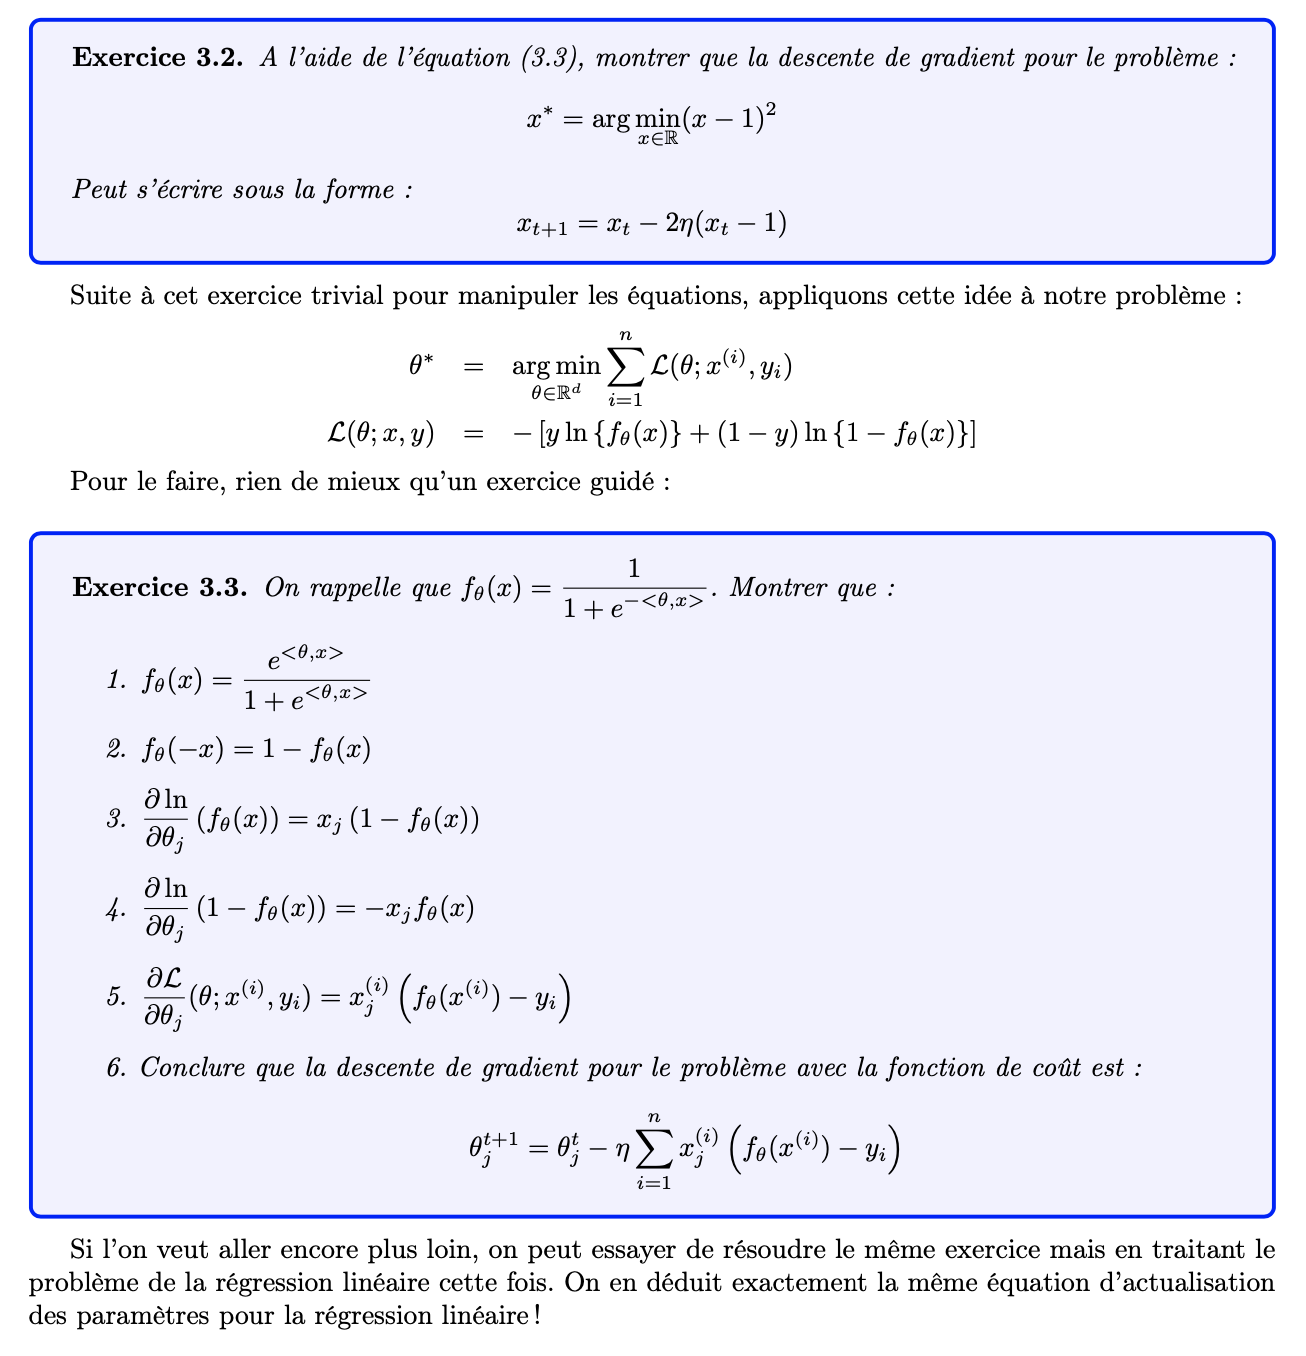
\includegraphics[width=\linewidth]{./img/notions_math/gradiant_descent/exercices}
